\vspace{-0.1in}
\section{Proposed Method}
\label{sec:Method Section}
\paragraph{Problem Statement} 
Let $\mathcal{D}^{train} = \{\left(\textbf{x}_i, \textbf{y}_i \right)\}_{i=1}^{N} \in \mathcal{P}^{train}$ denote the labeled training data from the source domain, where $\mathbf{x}$, $\mathbf{y}$ and $N$ represent the features, labels and data
amount, respectively. We consider two pre-trained source models, $f_{\theta_1}: \mathbf{x} \rightarrow \mathbf{y}$ and $f_{\theta_2}: \mathbf{x} \rightarrow \mathbf{y}$, parameterized by $\theta_1$ and $\theta_2$, respectively. These two models are well-trained on $\mathcal{D}^{\text{train}}$, and our goal is to adapt them to unlabeled, OOD target data in an online unsupervised manner. 

\vspace{-12pt}
\paragraph{Motivation} To fully exploit the potential of $f_{\theta_1}$ and $f_{\theta_2}$, a natural question arises: \textit{How do they benefit each other throughout the test-time adaptation process?} Unlike traditional paradigms such as the teacher-student framework~\cite{hu2022teacher}, ensemble learning~\cite{yang2023survey}, and multi-modal learning~\cite{yin2023crossmatch}, we aim to enable the models to mutually enhance each other in a bidirectional manner throughout the entire adaptation process. Additionally, the models share the same input and are designed for the same task. As shown in Fig.\ref{motifig1}, different models capture distinct facets of source knowledge due to variations in training strategies, architectures, or sizes—with larger models generally being more powerful. More importantly, Fig.\ref{motifig1} also reveals two key insights: 

\begin{itemize}

     \item \textbf{Different models offer complementary knowledge from training}.
     % In particular, these pre-trained models, even differing in sizes, can enhance one another by leveraging their respective confident predictions. 
     Though pre-trained models differ in sizes, they provide complementary confident knowledge to each other, which substantially enhances TTA performance. Taking ResNet-50 and ViT-Base as two peer collaborators, by harnessing the complementary knowledge from each other, the performance of ResNet-50 improves from 29.7\% to 34.6\%, while the performance of ViT-Base rises from 51.7\% to 56.9\% on ImageNet-C. 
     \item \textbf{Different models exhibit varying levels of robustness during TTA}. 
     % Smaller models often prove more resistant to misleading signals, which are inevitable and unpredictable in complex environments.
     While larger models are more accurate, smaller models can be more resistant to noisy learning signals, which commonly arise in complex TTA scenarios. 
     % In fact, when the adaptation process is misled by 2,250 incorrect labels, the performance of ViT-Base drops to a level comparable to that of ResNet-50.
     For example, when TTA is performed on 2,000 samples with incorrect pseudo labels, the performance of ViT-Base falls to a level even lower than that of ResNet-50.
\end{itemize}
% These observations highlight the promise of exploring cooperative adaptation mechanisms, although enabling stable co-adaptation between models of different sizes remains challenging due to the large gap of their outputs.
These observations underscore the potential of exploring cooperative TTA mechanisms. However, achieving stable co-adaptation between models of different sizes remains challenging, due to the substantial disparity in their outputs.


% vitb drop 28.1
% mobile drop 3.5
% 18 drop 3.2
% 50 drop 8.5
% 101 drop 11.7
% vits drop 2.1


% \paragraph{Motivation} Inspired from Fig.~\ref{motifig1}, different models capture different facets of source domain knowledge due to variations in training strategies, model architectures, or sizes. Notably, larger models tend to be more powerful. Despite these variations, two models can enhance one another by leveraging their complementary confident predictions. Moreover, their robustness varies when encountering erroneous information at test time, with smaller models generally being more resilient to incorrect guidance. This suggests that exploring cooperative mechanisms between different models throughout the adaptation process is promising. However, enabling effective co-adaptation between models of different sizes is challenging, as their outputs cannot be directly aligned.

% Therefore, our objective is to continuously adapt the two pre-trained source models to effectively handle each batch of target samples by leveraging cross-model co-learning. In this process, the two models complement each other, ultimately improving overall performance.
%After obtaining two pre trained models, due to the huge differences in parameter quantity, structure, and performance between the models, how to effectively utilize the knowledge of each model and enable them to collaborate? Meanwhile, since TTA focuses on the performance of the final model in the target domain, how can strong performance be demonstrated in the target domain after two models collaborate?
% In the context of test-time adaptation (TTA), a batch of unlabeled test samples arrives sequentially at each time step and is processed online without storage.
% \mathcal{X} \mathcal{Y}

% where two different source models $f_{\theta_1}\left(\textbf{x}\right)$ and $f_{\theta_2}\left(\textbf{x}\right)$ are utilized to represent the knowledge of the same domain. These two models mutually promote each other while they are simultaneously combined to better produce final predictions.
% To address this challenge, we propose a cross-model co-learning approach for TTA. Specifically, the two models $f_{\theta_1}$ and $f_{\theta_2}$ engage in mutual collaboration during adaptation. At each time step, the models share adaptation cues and insights derived from the unlabeled test data, enabling bidirectional knowledge exchange. This interaction allows each model to leverage the complementary strengths of the other, enhancing their ability to adjust to the distributional shifts between $\mathcal{P}^{\text{train}}$ and $\mathcal{P}^{\text{test}}$. Ultimately, we combine the adapted models to produce improved predictions on the test data. By integrating the strengths of both models through cross-model co-learning, our approach aims to achieve superior performance compared to traditional single-model TTA methods.

\begin{figure}[t]
\centering
    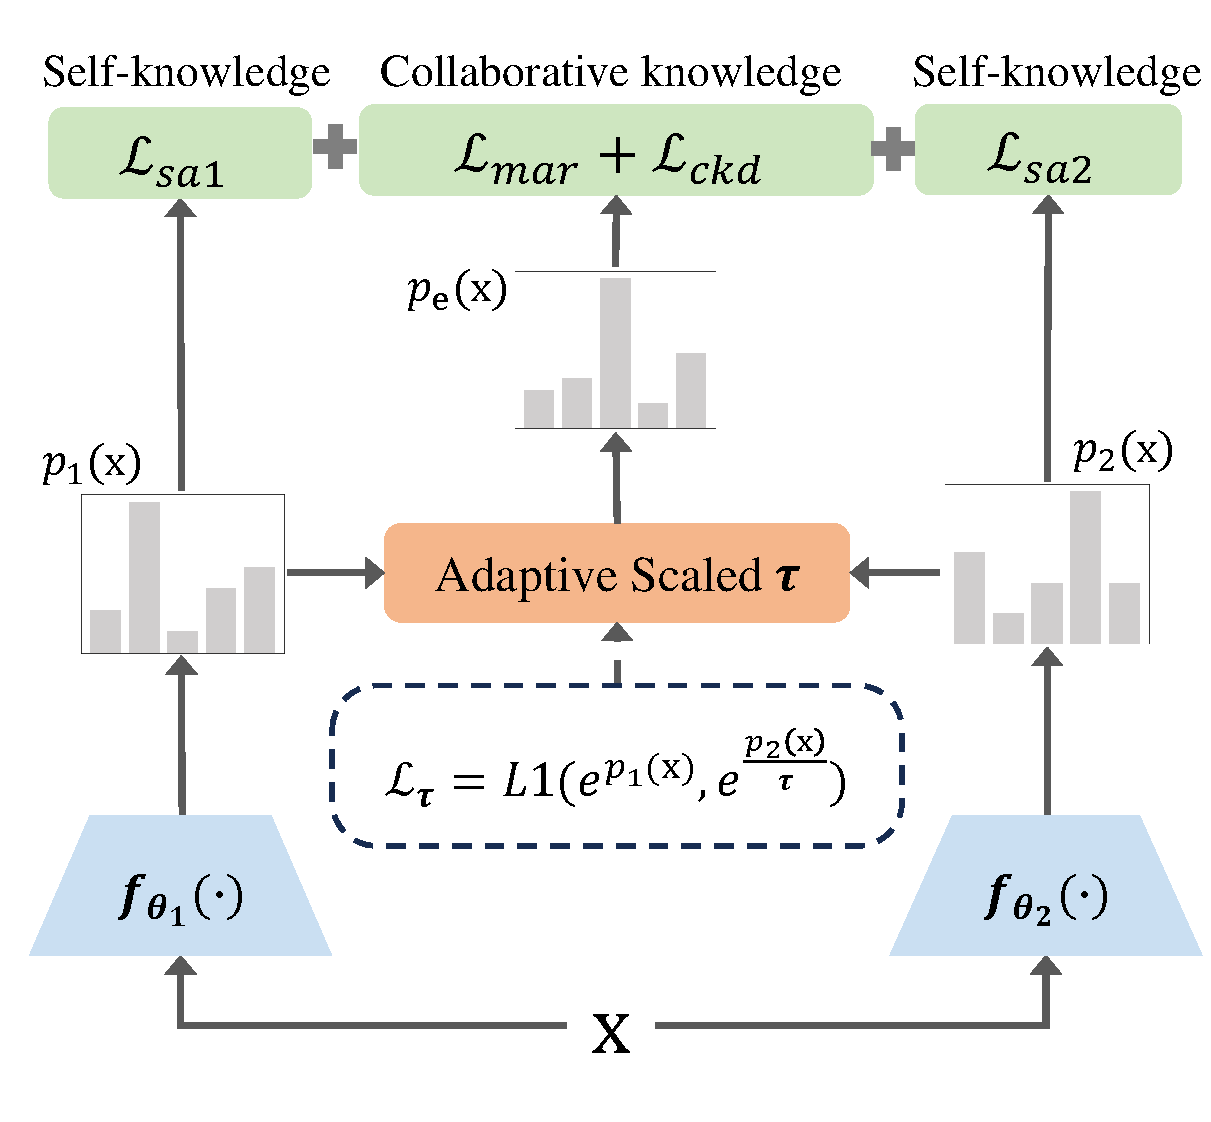
\includegraphics[width=0.93\linewidth]{sec/overview_3.7.pdf}
    % \vspace{-0.05in}
    \caption{The overall COCA framework consists of two models that adapt by leveraging both their inherent self-knowledge and the adaptive collaborative knowledge shared between them. To facilitate a more effective and robust ensemble of their outputs—namely, $p_1(\bx)$ and $p_2(\bx)$—a learnable parameter, $\tau$, is introduced. In this example, we designate $f_{\theta_2}$ as the auxiliary model, and its output is divided by $\tau$ to enable co-learning.}
    % A learnable parameter, $\tau$, is introduced to more effectively ensemble the outputs of the two models. The final predictions, $p_{com}(x)$, are derived from the combined outputs of both models.
    \vspace{-0.15in}
\label{overview}
\end{figure}


% The overall framework of COCA. Each model adapts by leveraging both its own self-knowledge and the adaptive collaborative knowledge shared with the other model. A learnable parameter, $\tau$, is introduced to enable a more effective and robust ensemble of the models' outputs, i.e., $p_1(\bx)$ and $p_2(\bx)$. In this example, we use $p_2(\bx)$ to represent the auxiliary model and the output of $p_2(\bx)$ will be divided by $\tau$.


\vspace{-11pt}\paragraph{Overall Framework} To leverage the unique strengths of different pre-trained models and address their varying robustness during test-time adaptation (TTA), we propose COCA, a cross-model co-learning approach that emphasizes an adaptive bidirectional cooperation mechanism. COCA employs two key strategies: co-adaptation and self-adaptation. The co-adaptation strategy harnesses the collaborative knowledge between models to mitigate individual biases during TTA, with adaptive alignment of outputs from models of different sizes further enhancing robustness. In contrast, the self-adaptation strategy refines each model’s unique strengths through unsupervised learning, enabling diverse and flexible adaptation to the target domain. An overview of COCA is shown in Fig.~\ref{overview}, and the corresponding pseudo-code is provided in Appendix~\ref{pscode}.

% \paragraph{Differences with Existing Paradigms}
% Our proposed COCA differs from existing TTA methods by emphasizing collaborative improvement between models. Unlike the traditional teacher-student framework~\cite{hu2022teacher, beyer2022knowledge}, where knowledge is transferred solely from a stronger teacher to a weaker student, COCA operates in a bidirectional manner, aiming to enhance overall performance while mutually improving both models. The robustness of COCA is ensured by the collaborative integration of the distinct advantages offered by different models. The key distinction between COCA and multi-modal~\cite{yin2023crossmatch} settings is that, in COCA, all models share the same input and task. In contrast to ensemble learning~\cite{yang2023survey}, where models typically make independent predictions that are later aggregated, COCA enables direct inter-model influence throughout the adaptation process, promoting deeper collaboration and dynamic knowledge exchange. By extending the performance boundaries of each model, we aim to achieve more effective real-time adaptation.

% \paragraph{Overall Framework} To exploit the diverse strengths of different pretrained models, we propose COCA, a cross-model co-learning approach for test-time adaptation (TTA). The overall details of COCA are illustrated in Fig. \ref{overview}. The key idea of our co-learning mechanism includes two strategies: i) exploiting model-specific knowledge through self-supervised learning, and ii) investigating collaborative information to further enhance each model. Predictions from both adapted models are adaptively aggregated to gain the final performance on the target domain.



% \begin{equation}\label{eq3}
% \begin{aligned}
%     \mathcal{L}_{se}=\min_{\theta}{\sum E(x)\over{\sum_{\mathbb{I}_{\{E(x; \theta)<E_0\}}x}}}.
% \end{aligned}
% \end{equation}

% The necessity of introducing the adaptive scaled temperature $\tau$. \emph{Average} refers to directly combining the outputs of the two models by averaging them to form collaborative knowledge.
\begin{figure*}[t]
\centering
    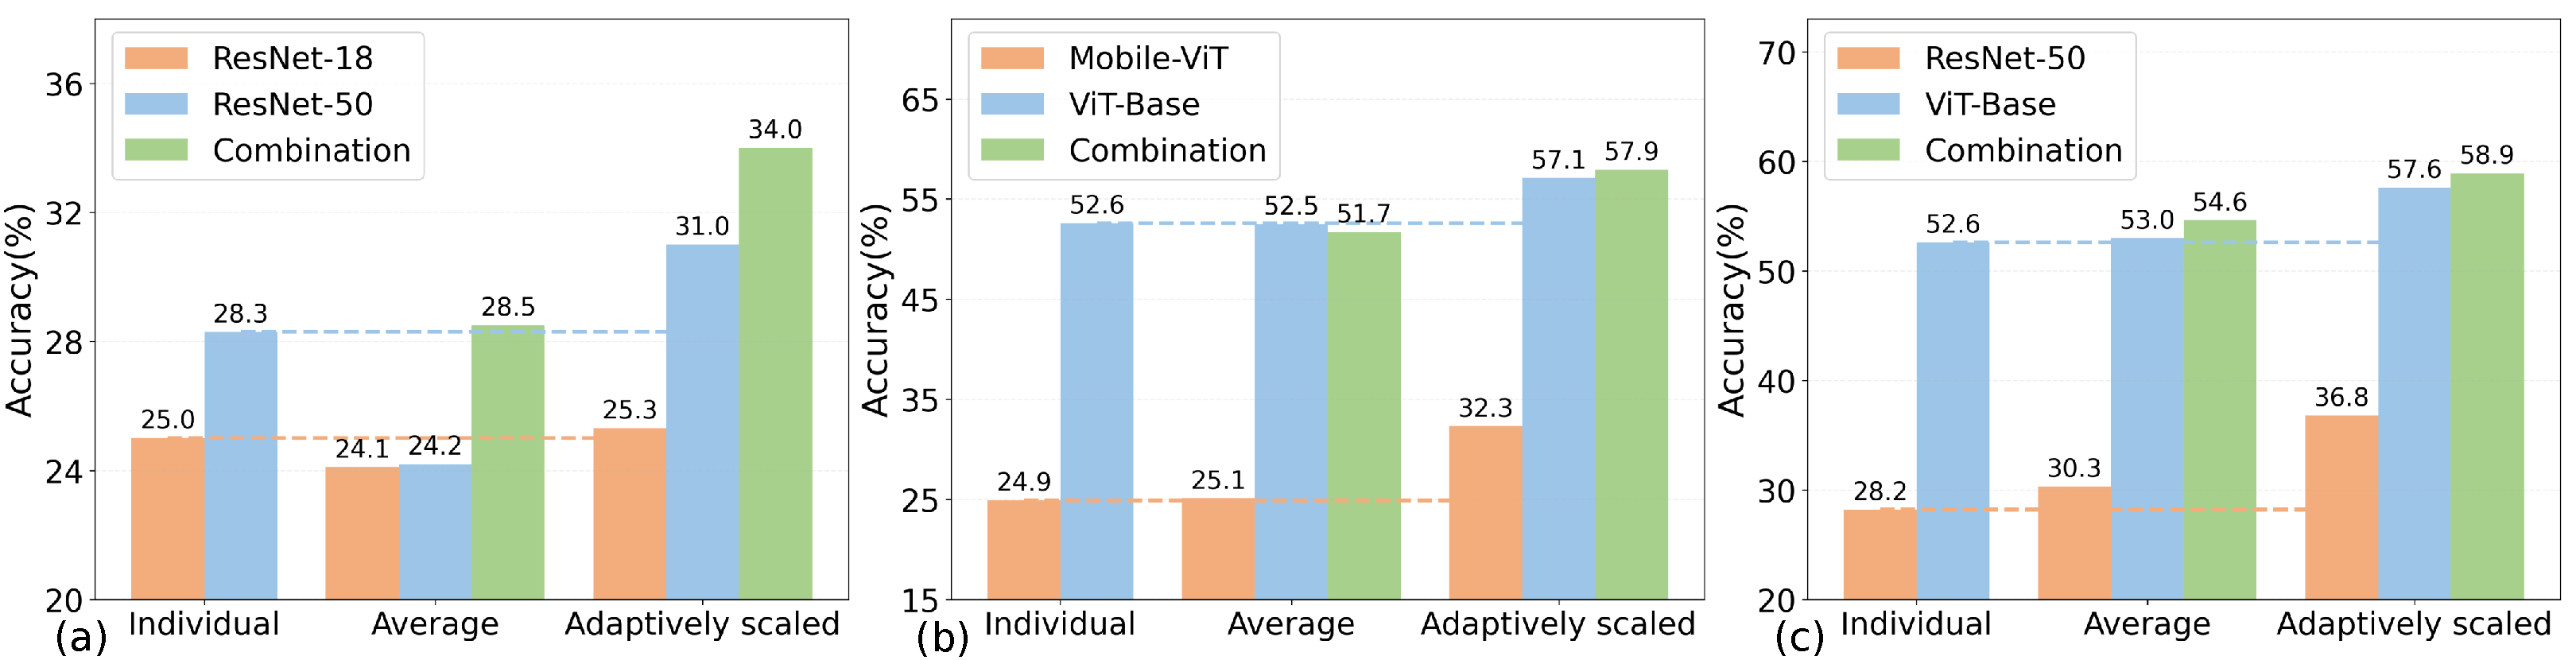
\includegraphics[width=\linewidth]{sec/Tcompare.pdf}
    \vspace{-0.25in}
    \caption{The necessity of introducing $\tau$, a learnable parameter. All experiments are based on Tent~\cite{wang2020tent}. \textit{Individual} refers to adapting each model independently, as done in Tent. \textit{Average} involves combining the predictions of two models by averaging their output logits for marginal entropy minimization. Under this strategy, the performance improvement is limited. In contrast, \textit{Adaptively scaled} utilizes the parameter $\tau$ to adaptively combine the output logits, resulting in a substantial increase in overall performance. }
    \vspace{-0.1in}
\label{Tcompare}
\end{figure*}


\subsection{Cross-Model Collaborative Adaptation} 
\label{aoi}
\label{tintro}
% overfitting
% We design COCA to integrate the complementary strengths from different models for test-time adaptation. This is important. This is challenging.
Unlike traditional TTA methods that depend solely on the limited knowledge of a single pre-trained model, our approach focuses on enhancing TTA performance and stability through cross-model collaboration. This collaborative strategy is particularly vital in the context of online unsupervised adaptation, where individual models are prone to overfitting their inherent biases and accumulating errors, as demonstrated in Table~\ref{mainres}. 

% Furthermore, we must consider two key factors, i.e., different models offer complementary knowledge from training, and different models exhibit varying levels of robustness during testing.
% To address that, our co-adaptation strategy focuses on aggregating the complementary knowledge from different models to enhance TTA. 
However, co-learning between models during testing presents significant challenges, due to both 1) varying degrees of miscalibration~\cite{naeini2015obtaining, tomani2021post} and 2) notable performance gaps in model predictions when handling OOD data. Consequently, simply averaging the outputs of multiple models for TTA can degrade overall performance, as in Fig.~\ref{Tcompare}.

% for knowledge aggregation
To make co-learning feasible at testing, we introduce a learnable diversity-aware scaling factor, $\tau$, which facilitates robust knowledge aggregation between large and small models for TTA. Specifically, in COCA, we identify the model with the larger parameter size as the \textit{anchor model}, and the other as the \textit{auxiliary model}, where larger models typically exhibit better in-distribution and out-of-distribution generalization~\cite{kim2023reliable}. 
During testing, we measure the discrepancies between the anchor predictions and the auxiliary predictions, which informs how trustworthy the auxiliary predictions are to determine the value of $\tau$. Formally, given anchor predictions logits $p_{a}(\bx)$ and auxiliary predictions logits $p_{s}(\bx)$, our goal is to learn a scaling factor $\tau$ in a unidirectional manner, so that:

\begin{equation}
    \arg \min_{\tau} \mathcal{L}_{s}(p_{a}(\bx), \frac{p_{s}(\bx)}{\tau}),
    \label{tloss}
\end{equation}
where $\mathcal{L}_{s}$ is a discrepancy function. Here, we adopt L1 loss to estimate this discrepancy, while projecting the prediction logits to the exponential space for discrepancy calculation, inspired by softmax. Then, $\mathcal{L}_{s}$ is formulated by:

\begin{equation}
    \mathcal{L}_{s}(p_a(\bx), p_s(\bx)) = \left |\left|e^{p_{a}(\bx)} - e^{p_{s}(\bx)} \right|\right|_1.
\end{equation}

We use this discrepancy loss to optimize \textit{only} the learnable factor $\tau$, and subsequently leverage $\tau$ for prediction aggregation, with the overall prediction $p_{e}(\bx)$ given by:
\begin{equation}
    p_{e}(\bx) = \frac{p_{e}'(\bx)}{T},~~\text{where}~p_{e}'(\bx)=p_{a}(\bx) + \frac{p_{s}(\bx)}{\tau}.
    \label{tau_ensemble}
\end{equation}
The learnable parameter $\tau$ serves to align the outputs of models with different sizes, thereby ensuring a more effective and robust adaptation process. The ensemble prediction is then utilized for marginal entropy minimization. Here, we introduce an adaptive balance factor $T$, defined as $\max p_{e}'(\bx) / \max p_{a}(\bx)$, to keep the max predictive logit unchanged after aggregation, maintaining a reasonable sharpness of $p_{e}(\bx)$.
Notably, the scaling factor $\tau$ does not modify the results of $p_{s}(\bx)$ but controls its contribution to the ensemble prediction $p_e(\bx)$ according to its reliability. \linebreak Experiments in Fig.~\ref{Tcompare} demonstrate the effectiveness of our $\tau$ to facilitate co-learning among models of various architectures and with different performance gaps.

% that adaptively integrates knowledge from different models
Based on the ensemble prediction $p_{e}(\bx)$, we construct the cross-model co-adaptation objective of COCA as:
\begin{equation}
\label{colloss}
    \mathcal{L}_{col} = \mathcal{L}_{mar} + \mathcal{L}_{ckd},
\end{equation}
with $\mathcal{L}_{mar}$ to enhance the separability of data in the ensemble prediction $p_e(\bx)$  and $\mathcal{L}_{ckd}$ to improve each model through knowledge distillation. We depict them below.
% We describe these components in more detail below. 
% with $\mathcal{L}_{mar}$ to enhance the separability of data in the ensemble prediction $p_e(\bx)$  and $\mathcal{L}_{ckd}$ to distill the integrated knowledge into each model. We depict them below.

\vspace{-5pt}\paragraph{Marginal Entropy Minimization} To improve the generalization of $p_e(\bx)$, our goal is to enhance the predictive confidence of $p_e(\bx)$, thereby learning a decision boundary that lies in the low-density sample region~\cite{grandvalet2004semi}. Following Tent~\cite{wang2020tent}, we adopt the entropy objective and apply it to $p_e(\bx)$ for marginal entropy minimization, defined as:
\begin{equation}
    \mathcal{L}_{mar} = - \sum_{c=1}^C p_{e}^c(\bx)\log p_{e}^c(\bx),
    \label{marginalent}
\end{equation}
where $C$ represents the number of categories.
% thereby learning a decision boundary that lies in the low-density region of the sample distribution

\vspace{-10pt}\paragraph{Cross-Model Knowledge Distillation}
In addition to $\mathcal{L}_{mar}$ that enhances the overall prediction performance, we also introduce a knowledge distillation loss to provide more direct learning signals, transferring knowledge from $p_{e}(\bx)$ to each individual model. This maximizes the utilization of cross-model knowledge in $p_e(\bx)$, and improves the generalization of each model. Specifically, we derive pseudo-labels from $p_e(\bx)$ and compute a cross-model knowledge distillation loss for each model based on cross-entropy loss: 
\begin{align}
\label{ckdloss}
\mathcal{L}_{ckd} = \mathcal{L}_{CE}(p_a(\bx),\hat{y}) + \mathcal{L}_{CE}(p_s(\bx),\hat{y}),
\end{align}
where $\hat{y}= \argmax p_e(\bx)$ denotes the pseudo-label of the ensemble prediction $p_e(\bx)$.
% to enhance the generalization of each model with more direct guidance signals
% We enhance the generalization of each model, by conducting knowledge distillation from $p_{e}(\bx)$ to the individual outputs. This xx , and thus enable a more robust TTA.
% distilling the ensemble knowledge for 

% To facilitate the flow of knowledge from the ensemble predictions to the individual models, we introduce pseudo-labels derived from the ensemble prediction $p_e(\bx)$. Using these pseudo-labels, we compute a Cross-Model Knowledge Distillation loss for each model, based on Cross-Entropy Loss:



% In the context of model co-learning, the asymmetric nature of different model architectures results in varying capacities for knowledge representation and adaptation. Generally, models with a larger number of parameters exhibit greater representational power and enhanced adaptation capabilities. When fostering collaboration among models, it is crucial to account for these differences in model capacity and adaptation potential. Motivated by this insight, we introduce the concept of an \textbf{anchor model} to establish a hierarchical collaboration framework. 

% Specifically, given two models: anchor model $f_{\theta_1}$ and non-anchor model $f_{\theta_2}$, we designate the model with more parameters as the anchor model, which serves as the primary guide during the test-time adaptation process. This design choice is founded on the intuition that the anchor model's broader knowledge base can provide more reliable adaptation directions.

% To facilitate effective knowledge transfer while preserving the complementary strengths of both models, we introduce an adaptive temperature scaling mechanism for the non-anchor model. Let $\tau$ be a learnable parameter that modulates the contribution of the non-anchor model without altering its fundamental predictions. The temperature scaling is applied as:

% \begin{equation}
% \tilde{p_2}(x) = \frac{p_2(x)}{\tau},
% \end{equation}
% where $p_2(x)$ represents the original logits of the non-anchor model $f_{\theta_2}$ and $\tilde{p_2}(x)$ denotes the logits after temperature-scaling.


% The parameter $\tau$ is optimized to minimize the distributional discrepancy between the two models:
% \begin{equation}\label{eq3}
% \begin{aligned}
%     L_{\tau }= \frac{1}{N} \sum_{i=0}^{N} \left |  e^{p_{1_{i}}(x)} - e^{\tilde{p_{2_{i}}}(x)} \right | ,
% \end{aligned}
% \end{equation}
% where $p_{1_{i}}(x)$ and $p_{2_{i}}(x)$ denote the logits of the $i$-th class(total $N$ classes) from the anchor and non-anchor models respectively and $|\cdot|$ denotes the L1 distance. 

% This loss function only optimize the adaptive temperature $\tau$ which encourages alignment between the two models output logits while maintaining their individual characteristics. Through this anchor-guided temperature scaling, we establish an asymmetric yet complementary collaboration between the two models, where the anchor model provides reliable adaptation guidance while the non-anchor model contributes supplementary knowledge through temperature-modulated predictions. In fig~\ref{Tcompare}, We conducted co learning experiments by combining the outputs of models with different structures and sizes and utilizing the combined outputs which Demonstrated the effectiveness and necessity of adaptive temperature scaling mechanism based on anchor model.






% \subsection{Cross-Model Knowledge Synthesis}
% In a collaborative framework, the outputs of two models naturally have differences and consensus parts. In order to effectively utilize the cross-model knowledge represented by the differences and consensus between model outputs, we divide the collaboration part into the following two parts based on the consistency of model behavior:
% \subsubsection{Discrepancy Cognition}
% \label{discog}
%  Firstly, we combine the predictions from both models through scaled averaging, where the non-anchor model's predictions are modulated by the learned temperature scaling mentioned in Section \ref{aoi}:

% \begin{equation}
%     p_{com}(x) = \frac{1}{2}(p_1(x) + \frac{p_2(x)}{\tau})
% \end{equation}


% After output combination, We introduce a marginal entropy minimization objective~\cite{zhang2022memo} that encourages more confident predictions. This marginal entropy minimizes the uncertainty across all categories of a sample in the combined prediction. To illustrate, consider a binary classification problem: if Model 1 output is [0.7, 0.3] and Model 2 output is [0.6, 0.4], with the combined output being [0.65, 0.35], the change in  combined probabilities reflects the differing behaviors of the two models. In the process of minimizing entropy on the combined output to encourage confident predictions. Specifically, when the highest class probability decreases and the probabilities of other classes increase, the direction of model updates shifts compared to before. Thus, the disparity between the two models directly influences the TTA process in the marginal entropy minimization. The marginal entropy can be expressed as:

% \begin{equation}
%     \mathcal{L}_{mar} = -\frac{1}{N}\sum_{i=1}^N \sum p_{com}(x)\log(p_{com}(x)).
%     \label{marginalent}
% \end{equation}
% where $N$ is the batch size. This marginal entropy minimization term drives the combined outputs toward more decisive predictions while naturally allowing the temperature-scaled anchor model to guide the model knowledge fusion through the modulation factor $\tau$.


% \subsubsection{Consensus Knowledge Extraction}
% \label{cons}
% Given the combined logits $p_{com}(x)$ from our cross-model framework as described in Section \ref{discog}, We hope to extract consensus knowledge between two models from the consistency of their predictive behavior. To illustrate, consider the same binary classification problem in Section \ref{discog}: if Model 1 outputs [0.7, 0.3] and Model 2 outputs [0.6, 0.4], with the combined output being [0.65, 0.35]. Although the two models have different entropy levels, they exhibit predictive consistency on class 0. Therefore, using pseudo labels corresponding to the maximum class probability of the combined output reflects the consistency of the predictions of the two models.


% At the same time, a natural question arises: what would happen if the predicted behavior of two models is completely inconsistent, resulting in a change in the final combined output? When the predictions of two models differ greatly, then due to the existence of automatic temperature scaling mentioned in Section \ref{aoi} , the contribution of non anchored models to the combined output will become very small, and anchored models will occupy a dominant position in the output combination.

% % To formalize this intuition, we first compute the prediction entropy of the combined probability distribution $E(p_{com})$ by Eqn.\ref{marginalent}.
% % where $p_{com}(x)^i$ represents the probability of class $i$. The entropy measure $E(p_{com})$ provides a theoretically-grounded assessment of prediction uncertainty, with lower values indicating stronger model agreement and higher confidence.
% % Based on this measure, we construct a reliability-filtered set $\mathcal{S}_{cons}$ :
% % \begin{equation}
% % \mathcal{S}_{cons} = \{x | E(p_{com}(x)) <  E_{0}\}
% % \end{equation}

% % For samples in $\mathcal{S}_{cons}$, we generate pseudo-labels through maximum likelihood estimation:
% To formalize this intuition, we first compute the pseudo-labels of the Combined outputs:
% \begin{equation}
% \hat{y} = \text{argmax} \: p_{com}(x)
% \end{equation}

% Then, these pseudo-labels are used to compute a consensus distillation loss for each model which based on Cross-Entropy Loss :

% \begin{equation}
% \mathcal{L}_{cons} = -\frac{1}{N}\sum_{j=1}^M\sum_{i=1}^N \mathcal{L}_{CE}(p(x),\hat{y})
% \end{equation}
% where $M$ denotes the amount of models, $N$ denotes the batch size.

% % $\mathbb{N}$ is an indicator function that when class $i$ belongs to the pseudo-labels' class, if yes$\mathbb{I}=1$ other will  $=0$.

% After consensus knowledge distillation and ensemble-based marginal entropy minimization, the collaboration between models can be expressed by a formula as:
% \begin{equation}
%     \mathcal{L}_{col} = \mathcal{L}_{cons} +\mathcal{L}_{mar}
% \end{equation}

% % \subsection{Logit Margin Regularization}
% % In the context of test-time adaptation, the absence of explicit supervision coupled with entropy minimization can lead to overconfident yet potentially incorrect predictions. This phenomenon, known as model miscalibration, can severely impact the reliability of adaptation. Meanwhile, the collaborative TTA between models mainly relies on entropy minimization in our framework, which makes this problem necessary to be solved. To address this issue, we propose a logits margin regularization mechanism that maintains appropriate confidence levels by constraining the relative differences between logits values.

% % Specifically, for any given input $x$, let $\mathbf{z} = [z_1, ..., z_C]$ denote the logits output where $C$ is the number of classes. We define the maximum logit value as:

% % \begin{equation}
% %     z_{max} = \max_{c} z_c
% % \end{equation}

% % To prevent excessive confidence, we introduce a margin-based penalty that enforces a maximum allowable distance between any logit and the maximum logit:

% % \begin{equation}
% %     \mathcal{L}_{lmr} = \frac{1}{N}\sum_{i=1}^N\sum_{c=1}^C \max(|z_c^{(i)} - z_{max}^{(i)}| - \delta, 0)
% % \end{equation}
% % where $\delta$ is a predefined margin hyperparameter that controls the maximum permitted gap between logits, and $|\cdot|$ denotes the L1 distance. This regularization effectively prevents the model from becoming overconfident by maintaining a reasonable spread in the logit space.

% % \subsection{Adaptive Pace Alignment}
% % The inherent structural differences between the anchor and non-anchor models can lead to inconsistent adaptation speeds, potentially degrading the effectiveness of their collaboration. To address this discrepancy, we introduce an adaptive pace alignment mechanism that synchronizes the adaptation process of both models.

% % Given the temperature-scaled parameter $\tau$ from Section 3.4, we formulate a pace alignment loss that guides the non-anchor model to follow the adaptation pace of the anchor model:

% % \begin{equation}
% %     \mathcal{L}_{pa} = \tau^2 D_{KL}(p\|p_{anchor})
% % \end{equation}
% % where $D_{KL}(\cdot\|\cdot)$ represents the Kullback-Leibler divergence, and $p$, $p_{anchor}$ denote the probability distributions of the non-anchor and anchor models respectively. The squared temperature term $\tau^2$ adaptively adjusts the strength of alignment based on the current distributional discrepancy between the models.




% develop each model based their related knowledge 
% Adaptation Under Model's Self-knowledge
\subsection{Self-Adaptation with Individual Knowledge}
\label{se}

The co-learning objective $\mathcal{L}_{col}$ aims to enhance TTA by reducing individual model biases. However, it enforces a uniform optimization direction across all models, which may overlook their unique capabilities. To address this, we further refine each model by leveraging its inherent knowledge, enabling us to harness their unique strengths and promote diverse adaptation to the target domain.

To this end, inspired by conventional single-model TTA methods, COCA adapts an individual model through the self/un-supervised learning objectives. Here, for simplicity, we adopt the entropy minimization loss from Tent~\cite{wang2020tent} and define the self-adaptation objective for each model as:
\begin{equation}
    \mathcal{L}_{sa} = - \sum_{c=1}^C (p_{a}^c(\bx)\log p_{a}^c(\bx) + p_{s}^c(\bx)\log p_{s}^c(\bx)).
    \label{selfloss}
\end{equation}
Note that $\mathcal{L}_{sa} $ is not limited to simple entropy minimization and COCA can seamlessly integrate with more advanced single-model TTA solutions, as verified in Table~\ref{mainres}.

% Similar to conventional single-model TTA methods, COCA adapts a given model by leveraging its own knowledge through self-supervised learning objectives. The concept of entropy minimization in TTA was first introduced by Tent~\cite{wang2020tent}, with the goal of reducing the predicted entropy to maximize the confidence of the model's output.  Subsequently, entropy minimization-based TTA methods that rely on reliable sample screening, such as EATA~\cite{niu2022efficient}, SAR~\cite{niu2023towards}, and DeYO~\cite{lee2024entropy} have become widely adopted. In our approach, we adopt the simple entropy minimization strategy from Tent~\cite{wang2020tent} to extract each model's self-knowledge. Specifically, for each test sample $x$ $\in$ $\mathcal{D}^{test}$, its entropy is computed using:
% Similar to traditional TTA methods, COCA also requires the model to adapt by utilizing models' self-knowledge. The entropy minimization in TTA was first proposed by tent~\cite{wang2020tent}, and the entropy minimization strategy aims to minimize the predicted entropy, thereby maximizing the confidence of the output. Then, the entropy minimization TTA method based on reliable sample screening became mainstream(EATA~\cite{niu2022efficient}, SAR~\cite{niu2023towards}, and DeYO~\cite{lee2024entropy}). In our method, we only choose the simple entropy minimization strategy following Tent~\cite{wang2020tent} to extract models' self-knowledge. For each test sample $x$ $\in$ $\mathcal{D}^{test}$, its' entropy is computed using:
% \begin{equation}\label{eq1}
% \begin{aligned}
% & E(x) = \sum_{c=1}^C-p^c(x)\log{p^c(x)},\\
% \end{aligned}
% \end{equation}
% where $c$ denotes the class of logit $p^c(x)$ and $C$ denotes the number of categories.
 
%  Let $\theta$ denote the model parameters. We calculate the entropy of the test samples and minimize it as follows:
% \begin{equation}\label{eq3}
% \begin{aligned}
%     \mathcal{L}_{se}=\min_{\theta}{\sum E(x)}.
% \end{aligned}
% \end{equation}

In summary, COCA's overall optimization objective is the combination of the co-adaptation and self-adaptation objectives for all samples, which is formulated as:
\begin{equation}
\label{fullloss}
    \mathcal{L} =\mathcal{L}_{col} + \mathcal{L}_{sa}.
\end{equation}
We evaluate the effectiveness of each component in Table~\ref{ablation}, where each objective exhibits incremental improvement. We will discuss the influence of exploring the ratio between $\mathcal{L}_{col}$ and $\mathcal{L}_{sa}$ in Appendix~\ref{Ratio}.
% In Section~\ref{sec:Experimental Section}, we will conduct ablation experiments to evaluate the effectiveness of the different components in this objective function. We provide the pseudo-code for COCA in Appendix due to page limit constraints.


% Our empirical analysis shows that this consensus-based knowledge extraction can effectively improve the performance of the COCA framework. (Detailed ablation results in Section~\ref{sec:Experimental Section}).


